
\subsubsection{Windows}


Download Flash Tool: \url{http://www.espressif.com/sites/default/files/tools/flash_download_tools_v3.4.9.2_0.zip}\\

Nach dem Download des letzten Release des NONOS SDK und des Flash Tool m�ssen beide Archive entpackt werden.
Dann kann das Flash Tool "`ESPFlashDownloadTool\_v3.4.9.2.exe"' gestartet werden. Nun  muss die korrekte COM-Nummer ausgew�hlt und die Bautrate auf 115200 gestellt werden. Danach kann mit der Start Taste der ESP gesucht werden. Wenn dies erfolgreich ist werden verschiedene Daten der Platine ausgelesen und im Fenster angezeigt.\\
Dann k�nnen die verschienden Dateien der neuen Firmware aus dem "`bin"' Verzeichnis des NONOS SDKs ausgew�hlt werden. Zu jeder Datei muss noch eine Start-Adresse eingeben werden.\\
Beim ESP-01 (8~MBit) m�ssen die angegebenen Dateien und Adressen eingegeben und �bertragen werden.    

\begin{figure}[ht]
  \centering
  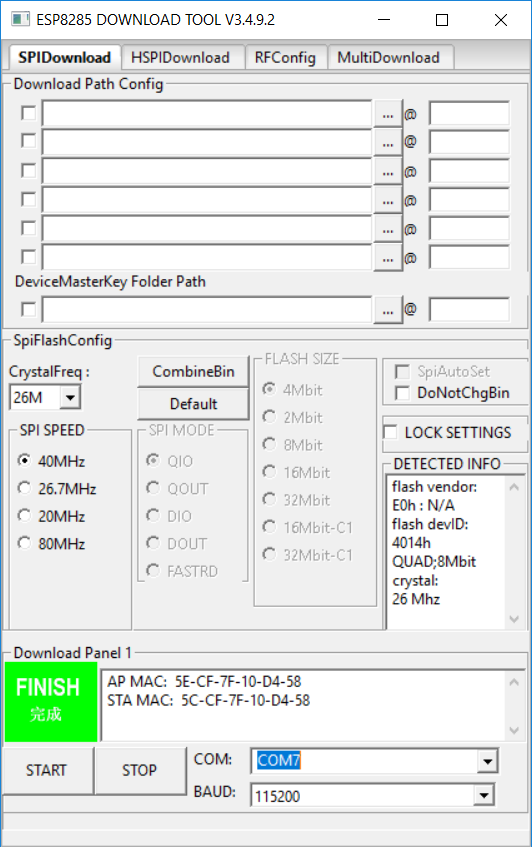
\includegraphics[scale=1.00]{images/ESP8266-ESP_01_FW_update_1.png}	
  %	\caption{}
  \label{ESP8266_ESP-01_FW_UPDATE_1}
\end{figure}

Danach kann mit der Start Taste die Aktualisierung gestartet werden. Wenn der blaue Balken das Ende erreicht hat, kann der ESP aus- und wieder angesteckt werden. Nun sollte die neue Firmware aktiv sein. Mit einem Terminalprogramm wie Putty (COM Verbindung) kann die Version abgefragt werden.

\begin{figure}[ht]
  \centering
  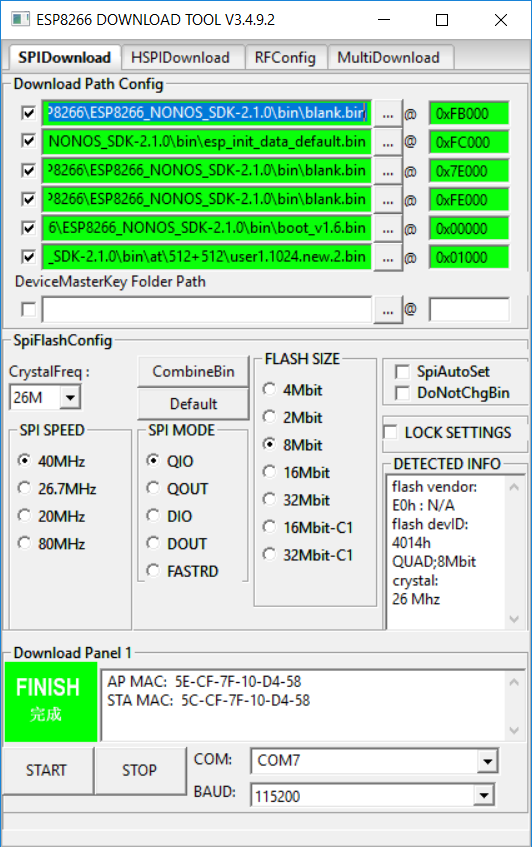
\includegraphics[scale=1.00]{images/ESP8266-ESP_01_FW_update_2.png}	
  %	\caption{}
  \label{ESP8266_ESP-01_FW_UPDATE_2}
\end{figure}


\begin{figure}[ht]
  \centering
  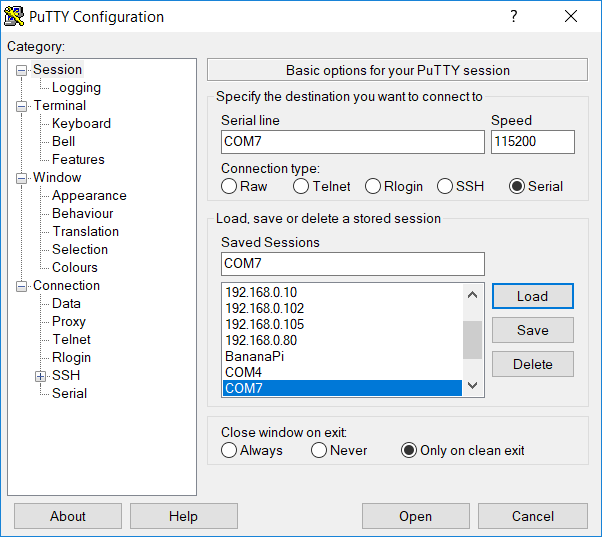
\includegraphics[scale=1.00]{images/Putty_COM.png}	
  %	\caption{}
  \label{Putty_COM}
\end{figure}

\begin{console}
Version abfragen: AT+GMR
\end{console}
\framebox{Enter} \framebox{Strg}+\framebox{J} 


\begin{screensmall}
AT version:1.4.0.0(May  5 2017 16:10:59)
SDK version:2.1.0(116b762)
compile time:May  5 2017 16:37:48
OK
\end{screensmall}

